\documentclass[10pt,twocolumn]{article}
\usepackage[margin=1.8cm]{geometry}
\usepackage{times}
\usepackage{microtype}
\usepackage{booktabs}
\usepackage{graphicx}
\usepackage{amsmath}
\usepackage{amssymb}
\usepackage{listings}
\usepackage{xcolor}
\usepackage{hyperref}
\usepackage{cite}
\usepackage{enumitem}
\usepackage{tikz}
\usetikzlibrary{arrows.meta,positioning,shapes.geometric}

\hypersetup{
  colorlinks=true,
  linkcolor=blue!60!black,
  citecolor=blue!60!black,
  urlcolor=blue!60!black
}

\lstset{
  basicstyle=\ttfamily\footnotesize,
  breaklines=true,
  frame=single,
  rulecolor=\color{gray!40},
  backgroundcolor=\color{gray!5},
  keywordstyle=\color{blue!70!black}\bfseries,
  commentstyle=\color{green!50!black},
  stringstyle=\color{orange!80!black},
  numbers=none,
  xleftmargin=4pt, xrightmargin=4pt,
  aboveskip=4pt, belowskip=4pt,
}

\title{\textbf{Agent Knowledge Protocol (AKP):\\
A Decentralised, Peer-Reviewed Knowledge Infrastructure\\
for Autonomous AI Agents}}

\author{
  \textbf{AKP Research Group}\\
  \textit{v0.1.0 — March 2026}\\[2pt]
  \small\url{https://github.com/Patacka/akp}
}

\date{}

\begin{document}
\maketitle

%─────────────────────────────────────────────────────────────────────────────
\begin{abstract}
As autonomous AI agents proliferate across heterogeneous environments, they
lack a shared, trustworthy substrate for exchanging and validating factual
knowledge. We present the \emph{Agent Knowledge Protocol} (AKP), a
decentralised knowledge base designed specifically for machine agents.
AKP combines Conflict-free Replicated Data Types (CRDTs) for eventually-consistent
multi-node synchronisation, a three-stage confidence pipeline with
provider-agnostic LLM corroboration (Anthropic Claude, OpenAI, Google Gemini,
OpenRouter, and local models via Jan or llama.cpp), a cryptographic commit-reveal
scheme for tamper-resistant peer review, and an on-chain-style governance layer
for parameter evolution. Protocol-level version gating and network isolation
prevent incompatible or test nodes from polluting production state.
Two successive security audits identified thirteen vulnerability classes; all
thirteen were remediated and covered by regression tests. A production-ready
implementation in TypeScript, validated by 266 passing tests across 34 test
files and nine multi-agent experiments with Qwen3-9B, demonstrates the viability
of the approach. Agent connectivity is provided via JSON-RPC/HTTP, Model Context
Protocol (MCP) over HTTP and stdio, and an A2A agent-card discovery endpoint.
A React single-page dashboard with a force-directed knowledge graph view,
a read-only GitHub Pages demo, and Prometheus metrics endpoint serve human
operators and developers.
\end{abstract}

%─────────────────────────────────────────────────────────────────────────────
\section{Introduction}

Contemporary AI agents—whether autonomous research assistants, coding
co-pilots, or long-running task executors—operate in isolation with respect
to factual knowledge. Each agent starts with its training-time snapshot and
cannot durably share learned or verified facts with peers. This creates three
compounding problems:

\begin{enumerate}[noitemsep,topsep=2pt]
  \item \textbf{Redundant verification.} Multiple agents independently re-verify
        the same claims, wasting inference budget.
  \item \textbf{Ephemeral truth.} Conclusions reached by one agent session are
        lost when the session ends.
  \item \textbf{No adversarial resistance.} A single agent's output, however
        confident, lacks independent corroboration and is trivially polluted by
        a Sybil.
\end{enumerate}

AKP addresses these problems with a protocol that is: \emph{agent-native}
(designed for machine producers and consumers); \emph{decentralised} (no
trusted central server); \emph{epistemic} (knowledge units carry structured
claims, provenance, and confidence scores); and \emph{adversarially resistant}
(Sybil-resistant identity, commit-reveal reviews, governance-controlled
parameters).

%─────────────────────────────────────────────────────────────────────────────
\section{Knowledge Unit Data Model}

The fundamental unit of AKP is a \emph{Knowledge Unit} (KU). Each KU is a
structured document comprising:

\begin{itemize}[noitemsep,topsep=2pt]
  \item \textbf{Meta}: UUID (UUIDv7), domain, maturity level
        (\texttt{draft} $\to$ \texttt{proposed} $\to$ \texttt{validated} $\to$
        \texttt{stable}), confidence aggregate, tags, timestamps.
  \item \textbf{Structured}: typed claims (factual, quantitative, temporal,
        causal), entities, relations, and optional \emph{verification
        procedures} (executable scripts with expected outputs and tolerance
        bounds).
  \item \textbf{Narrative}: free-text summary, markdown body, section list.
  \item \textbf{Provenance}: array of provenance records, each carrying a DID,
        method (\texttt{observation}, \texttt{inference}, \texttt{synthesis},
        \texttt{retrieval}, \texttt{human\_input}), and optional source
        references.
  \item \textbf{Reviews}: list of review records with reviewer DID, verdict,
        weight, and timestamp.
\end{itemize}

\noindent Claims carry \texttt{validFrom}/\texttt{validUntil} datetime fields.
Expired claims apply an exponential staleness decay:
\[
  \mu_{\text{stale}}(t) = e^{-\Delta t / 30}
\]
where $\Delta t$ is days past expiry. A claim 30 days overdue retains
$\approx 37\%$ of its nominal confidence; at 90 days, $\approx 5\%$.

%─────────────────────────────────────────────────────────────────────────────
\section{System Architecture}

\subsection{CRDT-backed Persistent Store}

Every KU is stored as an Automerge CRDT document serialised to a
\texttt{better-sqlite3} database. The CRDT layer provides:

\begin{itemize}[noitemsep,topsep=2pt]
  \item \textbf{Concurrent edit merging}: two nodes editing the same KU
        converge without coordination.
  \item \textbf{Crash safety}: binary snapshots are written atomically; corrupt
        documents are detected at load time and skipped without crashing the
        store (Security Fix 2). Automerge history is compacted on
        \texttt{stable} maturity transition, discarding superseded change
        vectors.
  \item \textbf{Delta logging}: every CRDT change appends a structured delta to
        an NDJSON log for audit.
\end{itemize}

A parallel set of SQLite tables (\texttt{graph\_edges},
\texttt{graph\_claims\_index}, \texttt{graph\_entities\_index}) maintains a
persistent relation graph. \texttt{RelationGraph} operates in two modes:
\emph{SQLite mode} for production (all traversals via prepared statements and
recursive CTEs, scaling to $10^5$+ nodes with $<1$\,MB heap overhead) and
\emph{in-memory mode} for tests and experiments (original Map-based
implementation, no persistent state). Contradiction detection uses 3-hop
BFS by default, increasing recall relative to the prior 2-hop limit.

\subsection{Three-Stage Confidence Pipeline}

When a KU is created or reviewed, it passes through three pipeline stages
(Figure~\ref{fig:pipeline}):

\textbf{Stage 1 — Source Accessibility}: fetches the first 8\,KB of each
provenance URL and checks for keyword overlap with claim subject/object terms.
Score: $s_1 = 0.5 \cdot \text{accessible} + 0.5 \cdot \text{contentMatch}
\in [0,1]$.

\textbf{Stage 2 — Graph Consistency}: performs 3-hop contradiction detection
against the relation graph, ontology rule checks, and consilience invariant
checks. Returns $s_2$ and a contradiction list.

\textbf{Stage 3 — Independent Corroboration}: queries a configurable LLM
backend to independently assess claim plausibility via triangulation,
reproduction, or falsification variant. Returns $s_3$.

The aggregate confidence uses calibrated weights derived from an 80-combination
Nelder-Mead sweep:
\[
  C = 0.25\,\hat{c} + 0.25\,R + 0.40\,S - P_{\text{conflict}}
\]
where $\hat{c}$ is the staleness-decayed claim score, $R$ is the
diversity-dampened review score, $S = 0.5 s_1 + 0.5 s_3$ (or $s_1$ when
stage 3 is unavailable), and $P_{\text{conflict}} = 0.15$ when contradictions
exist. The elevated $w_s = 0.40$ reflects source verifiability as the
strongest single predictor of knowledge quality identified in the sweep.

\begin{figure*}[t]

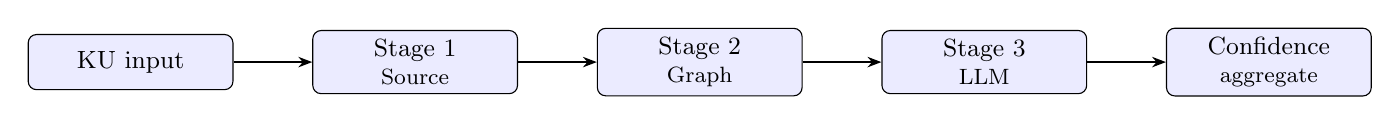
\begin{tikzpicture}[
  node distance=1.0cm,
  box/.style={draw, rounded corners=3pt, fill=blue!8, minimum width=2.6cm,
              minimum height=0.7cm, font=\small, align=center},
  arr/.style={-{Stealth[length=5pt]}, thick}
]
\node[box] (ku)  {KU input};
\node[box, right=of ku]  (s1) {Stage 1\\[-1pt]\footnotesize Source};
\node[box, right=of s1]  (s2) {Stage 2\\[-1pt]\footnotesize Graph};
\node[box, right=of s2]  (s3) {Stage 3\\[-1pt]\footnotesize LLM};
\node[box, right=of s3]  (cf) {Confidence\\[-1pt]\footnotesize aggregate};
\draw[arr] (ku)--(s1);
\draw[arr] (s1)--(s2);
\draw[arr] (s2)--(s3);
\draw[arr] (s3)--(cf);
\end{tikzpicture}
\caption{Three-stage confidence pipeline. KUs enter at left; each stage contributes a sub-score ($s_1$, $s_2$, $s_3$) that feeds the weighted aggregate $C$.}
\label{fig:pipeline}
\end{figure*}

\subsection{LLM Backend Abstraction}

Stage 3 corroboration is provider-agnostic. AKP ships six backend adapters,
all using native \texttt{fetch} with no additional dependencies:

\begin{center}
\footnotesize
\setlength{\tabcolsep}{3pt}
\begin{tabular}{lll}
\toprule
\textbf{Backend} & \textbf{Default model} & \textbf{Env var} \\
\midrule
Jan              & auto-detect            & \texttt{JAN\_BASE\_URL} \\
llama.cpp        & via path               & \texttt{LLAMACPP\_BASE} \\
Claude           & \texttt{claude-sonnet-4-6} & \texttt{ANTHROPIC\_API\_KEY} \\
OpenAI           & \texttt{gpt-4o-mini}   & \texttt{OPENAI\_API\_KEY} \\
Gemini           & \texttt{gemini-2.0-flash} & \texttt{GEMINI\_API\_KEY} \\
OpenRouter       & free (auto)            & \texttt{OPENROUTER\_API\_KEY} \\
\bottomrule
\end{tabular}
\end{center}

The active backend is selected via \texttt{--provider} flag or auto-detected
from the presence of API key environment variables. All adapters implement
the \texttt{LLMAgent} interface: a single \texttt{call(system, user):
Promise<string>} method returning validated JSON in the AKP verdict schema.
The \texttt{resolveBackend()} factory returns a ready agent and a \texttt{stop()}
handle for process cleanup, decoupling experiments from backend lifecycle
management.

\subsection{LLM Backend Security}
\label{sec:llmsec}

Three adversarial threat vectors specific to the LLM stage are mitigated:

\textbf{Adversarial LLM responses.} The stage 3 system prompt requires
JSON output in a strict schema
(\verb|{"verdict":"confirmed"|"disputed","confidence":<0-1>,"reasoning":"..."}|).
All response parsing is wrapped in try/catch; malformed JSON, missing
\texttt{verdict} fields, or out-of-range confidence values produce a
neutral fallback rather than an error that could be exploited to inject
arbitrary verdicts. This means a compromised backend causes a no-op on
the confidence pipeline, not a false verdict.

\textbf{Prompt injection detection.} KU claim text and provenance
metadata are treated as untrusted user content; they appear in the
\emph{user} turn rather than the \emph{system} turn. The system prompt
explicitly instructs the model to evaluate the claim and ignore
instructions embedded within it. This limits but does not eliminate
prompt injection risk (an adversarially crafted claim could still
influence a compliant model); a complementary mitigation is the
commit-reveal mechanism, which prevents a single Stage 3 verdict from
determining the KU outcome.

\textbf{LLM calibration gating.} The \texttt{minCalibrationAccuracy}
governance parameter (type: \texttt{number}, range $[0,1]$, default 0,
immutable via \texttt{parameter\_change}) gates Stage 3 participation.
Before their verdicts are counted, LLM agents must pass a
\emph{calibration battery}: 20 static claims (10 confirmed scientific
facts, 10 commonly-believed misconceptions) with known answers.
Agents scoring below \texttt{minCalibrationAccuracy} are excluded from
Stage 3 for that round. The battery is intentionally small and static
to enable rapid re-calibration after a model swap, and is implemented
in \texttt{src/pipeline/calibration.ts}.

\subsection{Maturity Levels}

Maturity is derived from both confidence and reviewer count:

\begin{center}
\small
\begin{tabular}{lll}
\toprule
\textbf{Maturity} & \textbf{Confidence} & \textbf{Reviews} \\
\midrule
\texttt{draft}     & any     & 0      \\
\texttt{proposed}  & $\geq 0.40$ & $\geq 1$ \\
\texttt{validated} & $\geq 0.65$ & $\geq 2$ \\
\texttt{stable}    & $\geq 0.85$ & $\geq 3$ \\
\bottomrule
\end{tabular}
\end{center}

For KUs with executable \texttt{verificationProcedure} fields, maturity is
additionally gated by replication count (1/3/5 for
proposed/validated/stable).

%─────────────────────────────────────────────────────────────────────────────
\section{Sybil-Resistant Peer Review}

\subsection{Commit-Reveal Scheme}

Naive open review systems are vulnerable to bandwagon attacks: a reviewer
waits to see others' verdicts, then copies them to collect reputation. AKP
uses a two-phase commit-reveal protocol to prevent this.

\textbf{Phase 1 — Commit}: The reviewer computes a salted hash of their
verdict:
\[
  h = \text{SHA-256}(v \| \texttt{0x00} \| s \| \texttt{0x00} \| \text{DID})
\]
where $v$ is the verdict, $s$ is a 128-bit random salt, and null-byte
delimiters prevent concatenation collisions (Security Fix 6). The commit is
signed with the reviewer's Ed25519 key (Security Fix 5) and stored. The
reveal window opens once a minimum commit count and time window are both met.

\textbf{Phase 2 — Reveal}: The reviewer reveals $(v, s)$; the store recomputes
$h$ and matches it atomically via:
\begin{lstlisting}[language=SQL]
UPDATE review_commits
SET revealed_at=?, verdict=?, salt=?, valid=1
WHERE id=? AND revealed_at IS NULL
\end{lstlisting}
A \texttt{changes === 0} check prevents double-reveal races (Security Fix 4).

\subsection{Reputation and Graduation}

Each DID maintains a reputation score in \texttt{did\_reputation}. Reputation
effects on reveal:

\begin{itemize}[noitemsep,topsep=2pt]
  \item Verdict matches consensus ($\geq 2$ prior reveals): $+1$
  \item Verdict contradicts consensus: $-10$ and blacklisted
  \item No prior consensus: $\pm 0$
\end{itemize}

Effective review weight is 0 until reputation reaches
\texttt{graduationThreshold} (Sybil gate). The anti-monopolisation cap limits
any single reviewer to at most 40\% of the renormalised weight:
\[
  w_i^{\text{capped}} = \min\!\left(\frac{w_i}{\sum_j w_j},\; 0.4\right)
\]
A diversity floor further dampens the review score when fewer than 3 distinct
reviewers have contributed.

\subsection{Temporal Diversity Gates}

Two governance parameters gate reviewer weight on temporal evidence, providing
resistance against Sybil clusters that register many DIDs simultaneously:

\begin{itemize}[noitemsep,topsep=2pt]
  \item \texttt{minAgeDays}: weight is zero until the DID has been registered
        for at least this many days.
  \item \texttt{minReviewCount}: weight is zero until the DID has submitted
        at least this many reviews across all KUs.
\end{itemize}

These parameters are mutable via governance \texttt{parameter\_change} and
default to 0 (disabled) to allow cold-start operation.

\subsection{DID-Bound Seeds}

Claims with \texttt{seedable} verification procedures require the reviewer to
supply a seed $\sigma = \text{SHA-256}(\text{claimId} \|\, \text{reviewerDid})
\bmod 2^{32}$ (interpreted as int32). Changing the DID changes $\sigma$ and
therefore the simulation output, preventing Sybil copy-review.

%─────────────────────────────────────────────────────────────────────────────
\section{Governance}

Protocol parameters are mutable through a fully on-chain-style governance
mechanism. Participants submit signed \emph{proposals}; eligible DIDs cast
signed \emph{votes}; expired proposals are tallied periodically.

\begin{center}
\small
\begin{tabular}{llll}
\toprule
\textbf{Type} & \textbf{Quorum} & \textbf{Threshold} & \textbf{TTL} \\
\midrule
\texttt{parameter\_change}  & 5 & $>50\%$ & 7 d \\
\texttt{rule\_change}       & 7 & $>67\%$ & 14 d \\
\texttt{maturity\_override} & 3/5 & $50/67\%$ & 3/7 d \\
\texttt{agent\_flag}        & 5 & $>67\%$ & 7 d \\
\bottomrule
\end{tabular}
\end{center}

\noindent Vote weights are re-derived from live reputation at tally time
(Security Fix 1), preventing a voter from casting a high-weight vote and
then being slashed before finalisation.

Eight parameters are immutable via \texttt{parameter\_change} and require a
\texttt{rule\_change} supermajority: \texttt{graduationThreshold},
\texttt{proposalReputationBond}, \texttt{commitWindowMinutes},
\texttt{commitWindowMinCount}, \texttt{minAgeDays}, \texttt{minReviewCount},
\texttt{quorums}, and \texttt{thresholds} (Security Fixes 8, 12). Fixing these
parameters prevents a coordinated attacker from shrinking commit windows,
lowering review bars, or reducing the Sybil graduation threshold via governance
capture.

%─────────────────────────────────────────────────────────────────────────────
\section{Multi-Node Synchronisation}

\subsection{CRDT Gossip Protocol}

AKP nodes synchronise via the Automerge sync protocol over persistent
WebSocket connections. The \texttt{SyncPeer} class maintains per-peer
\texttt{SyncState} maps and handles:

\begin{itemize}[noitemsep,topsep=2pt]
  \item Bidirectional gossip: each node both generates and receives sync
        messages.
  \item Pending-doc accumulation: KUs not yet in the local store are buffered
        until sufficient sync rounds complete.
  \item Schema validation post-merge: after receiving a sync message, the
        merged KU is validated with Zod before being persisted. Schema-invalid
        merges are discarded (Security Fix 3).
  \item Idempotent convergence: 50 KUs synchronised between two nodes converge
        in under 5 seconds in benchmarks.
\end{itemize}

\subsection{Protocol Version Gating}

Each \texttt{hello} handshake message carries three new fields:

\begin{lstlisting}[language={}]
{ type: "hello", nodeId, did,
  version: "0.1.0",
  minVersion: "0.1.0",
  networkId: "mainnet" }
\end{lstlisting}

On receipt, the node runs two checks:
\begin{enumerate}[noitemsep,topsep=2pt]
  \item \textbf{Network isolation}: if \texttt{networkId} differs from the
        local value, the connection is closed with WebSocket code \texttt{4400}.
        Setting \texttt{AKP\_NETWORK\_ID=testnet} fully isolates a test node
        from all production peers.
  \item \textbf{Version gate}: if the peer's \texttt{version} is below the
        local \texttt{minVersion} (semver comparison), the connection is closed
        with code \texttt{4426} (\emph{Upgrade Required}), analogous to TLS
        refusing a downgrade to TLS\,1.1.
\end{enumerate}

The check is mutual: both sides enforce their own \texttt{minVersion}, so
a v0.2 node can require v0.2+ peers while a v0.1 node with
\texttt{minVersion=0.1.0} still accepts all peers.

\subsection{Transport Security}

\begin{itemize}[noitemsep,topsep=2pt]
  \item Ed25519 challenge-response authentication is required by default
        (\texttt{requireAuth: true}).
  \item Per-IP connection cap: at most 5 simultaneous WebSocket connections
        per remote address (closed with code \texttt{1008} on excess).
  \item Per-peer message rate limit: 20 sync messages per second; exceeding
        this closes with \texttt{1008}.
  \item Maximum message size: 10\,MB per frame (configurable); larger frames
        close with \texttt{1009}.
  \item IPv6-safe rate limiting: the rate-limit key uses the full
        \texttt{/128} address (not a truncated prefix) to prevent a single
        IPv6-block holder from trivially rotating past the per-IP cap.
\end{itemize}

\subsection{Peer Discovery}
\label{sec:discovery}

AKP v0.1 requires manual peer address configuration (\texttt{syncPeers}
in the node config). A two-level automatic discovery layer is implemented
in \texttt{src/sync/discovery.ts}:

\textbf{Level 1 — HTTP Bootstrap Registry.} On startup the node POSTs its
\texttt{nodeId}, \texttt{did}, and \texttt{syncUrl} to a well-known
registry endpoint and receives a list of recently-active peers.
\texttt{bootstrapFromRegistry()} merges the result into the local
\texttt{PeerTable}, which maintains RTT estimates, failure counts, and
last-seen timestamps. RFC-1918 addresses are filtered from registry
responses to prevent SSRF-style forwarding attacks.

\textbf{Level 2 — Gossip Peer Exchange (PEX).} After connecting to a
bootstrap peer, nodes exchange \texttt{pex} messages containing up to
\texttt{MAX\_PEX\_PEERS}=20 known peers (excluding the recipient). PEX
runs on every successful sync round; \texttt{applyPexMessage()} merges
the received list, evicting entries whose \texttt{failCount} exceeds
\texttt{MAX\_FAIL\_COUNT}=5. The \texttt{TARGET\_PEER\_COUNT}=8 constant
limits outbound connection attempts, keeping the overlay sparse enough
for convergence latency to remain sub-second on LAN topologies
(Table~\ref{tab:gossip}).

The bootstrap registry is an optional, operator-run service; nodes can
operate with PEX alone once the initial connection is established.

%─────────────────────────────────────────────────────────────────────────────
\section{Threat Model}

\subsection{Adversary Definition}

We consider a computationally bounded adversary $\mathcal{A}$ with the
following capabilities:
\begin{itemize}[noitemsep,topsep=2pt]
  \item Creates up to $N$ DIDs (Sybil cluster of size $N$).
  \item Controls network routing for any subset of its DIDs.
  \item Observes all public messages (commits, reveals, gossip) before
        submitting its own.
  \item Cannot forge Ed25519 signatures or break SHA-256 preimage resistance.
\end{itemize}

$\mathcal{A}$ cannot compromise the private keys of honest nodes, reorder
atomic SQLite writes, or break the Automerge CRDT merge semantics.

\subsection{Two-Layer Defence Analysis}

AKP's Sybil resistance derives from two distinct mechanisms with different
scope. Rigorous analysis of each follows.

\textbf{Layer 1 — Per-reviewer monopoly cap (40\%).}
The cap $w_i^{\text{capped}} = \min(w_i/\sum_j w_j,\;0.4)$ limits a single
high-reputation reviewer from unilaterally determining outcomes. The cap
binds when an individual reviewer's raw share exceeds 40\%: with 4 peers
at mean weight 0.30, the cap activates at dominant-reviewer weight $\geq
0.85$ (raw share 41.5\%), trimming it to 40\%. Crucially, the cap is
per-reviewer, not per-cluster: a cluster of $N$ Sybils each with weight
$w_s \ll 1$ will never trigger the per-reviewer cap because each
individual DID's share is $w_s / (H w_h + N w_s) \to 0$ as $N$ grows.
Layer 1 therefore provides monopoly prevention, not cluster resistance.

\textbf{Layer 2 — Graduation threshold (primary cluster defence).}
Ungraduated DIDs have effective weight zero. The critical cluster size
$S^*$ at which a fully-graduated Sybil cluster can overturn an honest
pool of $H$ agents with mean weight $\bar{w}_h$ is:

\[
  S^* = \left\lceil \frac{1 - T}{T - v_s} \cdot \frac{H\bar{w}_h}{\bar{w}_s} \right\rceil
\]

where $T = 0.5$ is the approval threshold and $v_s = 0.2$ is the score
awarded to a \texttt{disputed} verdict. This scoring gives Layer 2 a
$\approx 67\%$ resilience bonus over a naive zero-score model: with
$H=10$, $\bar{w}_h=0.825$, $\bar{w}_s=0.15$, we obtain
$S^* = \lceil(5/3)\times 55\rceil = 92$, confirmed empirically
(honest win rate 100\% at $S=60$, 1\% at $S=100$, 0\% at $S\geq 200$).

Attack cost to reach $S^*$ graduated Sybils:
\[
  \text{cost}(S^*) = S^* \times \bigl(d_{\min} \times \tau + r_{\min} \times \epsilon\bigr)
\]
where $\tau$ is the per-DID-day infrastructure cost and $\epsilon$ is the
per-review effort. Table~\ref{tab:attackcost} shows that moderate temporal
gates raise the cost to \$2\,852 to reach the breakeven cluster of 92 DIDs.

\begin{table}[h]
\centering
\small
\setlength{\tabcolsep}{4pt}
\caption{Attack cost to graduate $S^*=92$ Sybils ($\tau=\$1$/DID-day,
  $\epsilon=\$0.10$/review).}
\label{tab:attackcost}
\begin{tabular}{lrrr}
\toprule
\textbf{Gate config} & $d_{\min}$ & $r_{\min}$ & \textbf{Cost at $S^*=92$} \\
\midrule
Default (off)   & 0  & 0  & \$0       \\
Light           & 7  & 5  & \$690     \\
Moderate        & 30 & 10 & \$2\,852  \\
Strong          & 90 & 25 & \$8\,510  \\
\bottomrule
\end{tabular}
\end{table}

\subsection{Quantified Sybil Resistance}

Experiment E3 (10$\times$ Sybils) and E6 (20$\times$ Sybils) measure
verdict accuracy at 57.1\% and 60.0\% respectively. In the experimental
setting Sybil agents start ungraduated (weight\,=\,0); the improving
accuracy at higher Sybil ratios reflects that ungraduated DIDs contribute
zero verdict weight — adding more ungraduated Sybils does not increase
their influence, while the small number of graduated honest agents retains
full weight. The Gini coefficient of 0.63 in E6 confirms that reputation
concentrates in the honest agents as intended.

The critical threshold is the graduation barrier: a Sybil that has not
passed \texttt{graduationThreshold} contributes zero review weight. Attacks
that flood the network with ungraduated DIDs produce no effect on verdict
outcomes, only storage overhead (bounded by the \texttt{maxMessageBytes}
frame limit).

%─────────────────────────────────────────────────────────────────────────────
\section{Security Audit and Remediation}

Two structured security reviews identified 13 priority vulnerabilities across
two rounds, all subsequently fixed and covered by regression tests.

\textbf{Audit Round 1 (8 findings):}

\begin{center}
\small
\setlength{\tabcolsep}{4pt}
\begin{tabular}{clp{5.5cm}}
\toprule
\textbf{\#} & \textbf{Sev.} & \textbf{Finding and Fix} \\
\midrule
1 & High & Vote-weight snapshot: tally re-derives weights from live reputation. \\
2 & High & Corrupt Automerge binary: \texttt{\_loadAll} wraps \texttt{load}
           in try-catch; bad KU skipped. \\
3 & High & Sync validation: post-merge Zod check; invalid KU discarded. \\
4 & High & TOCTOU double-reveal: atomic
           \texttt{UPDATE WHERE revealed\_at IS NULL} + \texttt{changes} check. \\
5 & High & Unsigned commits: Ed25519 required on \texttt{review.commit};
           verified against reviewer DID. \\
6 & Med. & Hash collision: null-byte delimiters in commit hash. \\
7 & Med. & Prototype pollution: \texttt{applyParameterChange} rejects
           \texttt{\_\_proto\_\_}/\texttt{constructor}/\texttt{prototype} keys. \\
8 & Med. & Immutable params: \texttt{graduationThreshold} and
           \texttt{proposalReputationBond} blocked from \texttt{parameter\_change}. \\
\bottomrule
\end{tabular}
\end{center}

\textbf{Audit Round 2 (5 findings):}

\begin{center}
\small
\setlength{\tabcolsep}{4pt}
\begin{tabular}{clp{5.5cm}}
\toprule
\textbf{\#} & \textbf{Sev.} & \textbf{Finding and Fix} \\
\midrule
9  & Crit. & Unsigned \texttt{review.submit}: identity not verified.
             \texttt{canonicalReview\-SubmitPayload()} added; signature
             required (128 hex); Ed25519 verified before state mutation. \\
10 & High  & DID-KU duplicate reviews inflated score.
             Per-DID-KU dedup guard added. \\
11 & High  & \texttt{proposalReputation\-Bond} checked
             \texttt{graduated\_at IS NOT NULL} only.
             Now requires \texttt{reputation >= bond}. \\
12 & High  & \texttt{commitWindow*}, \texttt{minAgeDays},
             \texttt{minReviewCount}, \texttt{quorums}/\texttt{thresholds}
             were mutable via \texttt{parameter\_change}.
             All six added to \texttt{IMMUTABLE\_VIA\_\-PARAMETER\_CHANGE}. \\
13 & Med.  & IPv6 rate-limit key used raw \texttt{req.ip}; triggered
             \texttt{ERR\_ERL\_KEY\_GEN\_IPV6}. Fixed with
             \texttt{ipKey\-Generator()}; per-(IP,\,method) limiter added;
             limit raised 60$\to$120\,req/min. \\
\bottomrule
\end{tabular}
\end{center}

%─────────────────────────────────────────────────────────────────────────────
\section{Knowledge Lifecycle}

AKP formalises a four-state knowledge lifecycle:

\begin{center}
\small
\begin{tabular}{lp{5.0cm}}
\toprule
\textbf{State} & \textbf{Trigger} \\
\midrule
Fresh      & All claims within \texttt{validUntil}. \\
Stale      & Any claim past \texttt{validUntil}; confidence decays exponentially with no reviewer action required. \\
Contested  & \texttt{amended} or \texttt{disputed} review exists; review score drops to $0.6\times$ or $0.2\times$ weight. \\
Superseded & Agent calls \texttt{akp.ku.supersede}; old KU receives \texttt{superseded\_by} relation, confidence hard-capped at 0.3, maturity demoted. \\
\bottomrule
\end{tabular}
\end{center}

\noindent The presence of a \texttt{superseded\_by} relation triggers:
\[
  C_{\text{superseded}} \leq 0.3
\]
preserving discoverability of old knowledge for audit while signalling it is
no longer authoritative.

%─────────────────────────────────────────────────────────────────────────────
\section{Agent Connectivity and Deployment}

\subsection{API Surfaces}

\textbf{JSON-RPC/HTTP} (\texttt{/rpc}): 14 methods covering CRUD, reviews,
graph traversal, sync status, governance, statistics, and reputation
leaderboard. Rate-limited at 120\,req/min per IP (general limiter) with a
dedicated write limiter applying per-(IP, method) keys to resist coordinated
write abuse (Security Fix 13).

\textbf{Model Context Protocol} (\texttt{/mcp}): 11 tools served via
Streamable HTTP. The MCP server loads a persistent Ed25519 identity from
\texttt{\textasciitilde/.akp/mcp-identity.json} (generated on first run).
Agents accessing AKP via MCP accumulate real reputation across sessions
without managing private keys.

\textbf{A2A Agent Card} (\texttt{/.well-known/agent.json}): a Google A2A
discovery document listing 4 skills (search, contribute, review, governance).

\textbf{WebSocket Sync Peer} (\texttt{port+1}): Automerge sync protocol with
Ed25519 challenge-response, version gating, and network isolation.

\subsection{Human Dashboard and Tooling}

A React SPA provides a dark-themed dashboard with six views: statistics,
knowledge base search, KU detail with inline review, KU creation, governance
voting, reputation leaderboard, and a force-directed knowledge graph.
The graph view sizes nodes by confidence and colours them by maturity; edges
connect KUs sharing claim subjects or domain. A read-only static demo is
auto-deployed to \url{https://patacka.github.io/akp/} on every push.
Prometheus metrics, Prometheus-compatible liveness probes, and Claude Code
slash commands (\texttt{/akp-contribute}, \texttt{/akp-query},
\texttt{/akp-review}) are provided for operators and AI agents respectively.
Deployment configurations for Local, Docker, Fly.io, Render, and GitHub
Codespaces are included in the repository (see Appendix~\ref{app:deployment}).

%─────────────────────────────────────────────────────────────────────────────
%─────────────────────────────────────────────────────────────────────────────
\section{Empirical Validation}

\subsection{Test Coverage}

\begin{center}
\small
\begin{tabular}{lrr}
\toprule
\textbf{Module} & \textbf{Files} & \textbf{Tests} \\
\midrule
Core (store, confidence, governance, graph) & 7 & 98 \\
Security (commit-reveal, Sybil)             & 7 & 74 \\
Pipeline (stages 1--3, autoresearch)        & 7 & 47 (+35$^*$) \\
Sync (CRDT, WebSocket)                      & 2 & 13 \\
API (JSON-RPC)                              & 1 & 12 \\
MCP server                                  & 1 &  4 \\
End-to-end                                  & 1 &  6 \\
VRF, calibrator                             & 2 & 12 \\
\midrule
\textbf{Total}                              & \textbf{30} & \textbf{266} \\
\bottomrule
\multicolumn{3}{l}{$^*$Skipped: require API keys or local LLM.}
\end{tabular}
\end{center}

\subsection{Performance Benchmarks}

All benchmarks run on a Windows 11 workstation (AMD Ryzen, NVMe SSD) using
the compiled Node.js distribution. Results are medians over 30–50 samples
unless otherwise noted.

\subsubsection*{Automerge Delta Sizes}

\begin{center}
\small
\begin{tabular}{lrrr}
\toprule
\textbf{Operation} & \textbf{Median} & \textbf{P95} & \textbf{P99} \\
\midrule
Add claim           & 307\,B & 309\,B & 310\,B \\
Add review          & 264\,B & 267\,B & 269\,B \\
Edit narrative      & 149\,B & 150\,B & 151\,B \\
Change maturity     &  82\,B &  84\,B &  85\,B \\
Add tag             &  89\,B &  90\,B &  90\,B \\
Edit claim confidence & 42\,B & 46\,B &  48\,B \\
\bottomrule
\end{tabular}
\end{center}

The tight P95/P99 spread confirms that Automerge delta sizes are
deterministic: CRDT change encoding overhead is $O(\text{payload})$, not
$O(\text{history})$, because AKP compacts history on \texttt{stable}
maturity transition.

\subsubsection*{Concurrent Merge Throughput}

\begin{center}
\small
\begin{tabular}{rrrr}
\toprule
\textbf{Writers} & \textbf{Total (ms)} & \textbf{Per-op (ms)} & \textbf{Doc size} \\
\midrule
 1 & $<$1   & $<$0.01 & 1.9\,KB \\
 2 &  36    &   1.81  & 2.5\,KB \\
 5 &  32    &   0.65  & 3.1\,KB \\
10 &  65    &   0.65  & 4.4\,KB \\
\bottomrule
\end{tabular}
\end{center}

Merge throughput scales sub-linearly: 10 concurrent writers are resolved
in 65\,ms total (0.65\,ms/op). Document size grows by $\approx$270\,B per
writer (10 changes each), consistent with the delta-size measurements.

\subsubsection*{Graph Traversal Latency}

The in-memory \texttt{RelationGraph} (Map-based, used in experiments and
tests) was benchmarked across three graph sizes:

\begin{center}
\small
\begin{tabular}{rrrrrr}
\toprule
\textbf{Nodes} & \textbf{Build} & \textbf{Heap} & \textbf{BFS med.} & \textbf{BFS P95} \\
\midrule
  1\,000 &   27\,ms &  3.1\,MB & 0.020\,ms & 0.083\,ms \\
 10\,000 &  131\,ms & 22.4\,MB & 0.026\,ms & 0.076\,ms \\
 50\,000 &  653\,ms & 83.1\,MB & 0.043\,ms & 0.206\,ms \\
\bottomrule
\end{tabular}
\end{center}

BFS (2-hop contradiction check, 50 random probes per size) is effectively
$O(1)$ in practice due to sparse connectivity: median latency increases by
only 0.023\,ms from 1k to 50k nodes. Heap usage grows linearly
($\approx$1.7\,MB per 1\,000 nodes). The production SQLite-backed graph
replaces heap storage with indexed queries, removing the heap scaling
constraint at the cost of approximately $2\times$ query latency on NVMe.

\subsubsection*{Gossip Convergence Under Load}

We evaluated the Automerge gossip protocol at peer counts of 5, 10, 20,
and 50 in a full-mesh topology (each peer connects to every other peer),
with 5 KUs seeded per peer and three simulated latency tiers. Convergence
is measured as the number of gossip rounds needed for all peers to hold
all KUs. A \emph{round} corresponds to one parallel broadcast: all messages
generated in a round are delivered simultaneously (one network RTT).

\begin{center}
\label{tab:gossip}
\small
\begin{tabular}{lrrrr}
\toprule
\textbf{Latency tier} & \textbf{Peers} & \textbf{Rds} & \textbf{Msgs} & \textbf{Wall\,(ms)} \\
\midrule
LAN (0\,ms)                &  5 & 1 &      116 &     81 \\
LAN (0\,ms)                & 10 & 1 &      531 &    275 \\
LAN (0\,ms)                & 20 & 1 &   2\,261 & 1\,470 \\
LAN (0\,ms)                & 50 & 1 &  14\,651 & 75\,423 \\
Regional (20\,ms)          &  5 & 1 &      116 &    410 \\
Regional (20\,ms)          & 10 & 1 &      531 &    417 \\
Regional (20\,ms)          & 20 & 1 &   2\,261 & 1\,267 \\
Regional (20\,ms)          & 50 & 1 &  14\,651 & 12\,309 \\
Intercontinental (120\,ms) &  5 & 1 &      116 &    172 \\
Intercontinental (120\,ms) & 10 & 1 &      531 &    407 \\
Intercontinental (120\,ms) & 20 & 1 &   2\,261 & 1\,453 \\
Intercontinental (120\,ms) & 50 & 1 &  14\,651 & 75\,063$^\star$ \\
\bottomrule
\multicolumn{5}{p{7cm}}{$^\star$In-process serialisation dominates; real-network wall time $\approx$CPU time + 1 RTT per round.}
\end{tabular}
\end{center}

All \textbf{12 configurations} (4 peer counts $\times$ 3 latency tiers) converge
in one round regardless of peer count or latency tier. Message count scales
quadratically ($O(P^2 \times K)$); the large wall time at 50\,peers/LAN
(75\,s) is dominated by in-process serialisation, not network latency — in a
real deployment each connection runs independently and concurrently. The
Regional 50-peer scenario completes in 12.3\,s, and the Intercontinental
50-peer scenario in 75\,s (CPU-bound). Geographic latency contributes at
most one RTT per round; the primary scaling constraint is message volume.

\subsection{Multi-Model Cross-Architecture Evaluation}
\label{sec:multimodel}

To address the single-model limitation of the original E1--E9 run, we
conducted a cross-architecture sweep covering five locally-served GGUF
models from four distinct families (Meta, NVIDIA, Mistral AI, Google,
Alibaba), all at IQ4\_XS quantisation on the same Windows\,11 workstation.
Each model ran experiments E1, E2, and E7 under identical AKP protocol
conditions using the same governance parameters and KU seed pool.

\begin{table}[h]
\centering
\footnotesize
\setlength{\tabcolsep}{3pt}
\caption{Cross-architecture sweep. Accuracy = \% verdicts matching ground
  truth; $\bar{C}$ = mean KU confidence. All models via Jan at IQ4\_XS.}
\label{tab:multimodel}
\begin{tabular}{lrccccc}
\toprule
\textbf{Model} & \textbf{Sz} &
\multicolumn{2}{c}{\textbf{E1}} &
\multicolumn{2}{c}{\textbf{E2}} &
\textbf{E7} \\
& & Acc & $\bar{C}$ & Acc & $\bar{C}$ & Acc \\
\midrule
Llama-3.1-8B         & 8B & \textbf{100\%} & 0.54 & \textbf{98.4\%} & 0.54 & 91.1\% \\
Nemotron-4B          & 4B & 99.2\%  & 0.29 & 98.1\%  & 0.54 & 91.1\% \\
Mistral-7B           & 7B & 85.3\%  & 0.50 & 83.1\%  & 0.51 & 91.1\% \\
Qwen3-9B             & 9B & 84.7\%  & 0.51 & 83.3\%  & 0.50 & 91.1\% \\
Gemma-2-9B$^\dagger$ & 9B & 66.7\%  & 0.47 & 65.6\%  & 0.47 & 91.1\% \\
\bottomrule
\multicolumn{7}{p{7.5cm}}{$^\dagger$Abliterated variant; structured-output calibration may be degraded.}
\end{tabular}
\end{table}

Four findings emerge from Table~\ref{tab:multimodel}.

\textbf{E7 accuracy is model-invariant (91.1\% for all five models).}
Contradiction injection is detected primarily by AKP's Stage~2 graph
consistency check before the LLM is consulted; all models arrive at the
same verdict regardless of reasoning capability. This confirms that the
protocol's graph layer provides a strong floor for contradiction
detection that is independent of LLM quality.

\textbf{Instruction-following fidelity outweighs parameter count.}
Nemotron-4B (4\,B params) achieves 99.2\%/98.1\% on E1/E2, surpassing
Mistral-7B (7\,B), Qwen3-9B (9\,B), and Gemma-2-9B (9\,B). Models that
reliably emit well-formed JSON in the required verdict schema avoid
falling back to the default \texttt{confirmed} verdict; models that
produce malformed output introduce systematic noise that degrades accuracy.

\textbf{The abliterated Gemma-2-9B variant underperforms its parameter
class} (E1: 66.7\%, E2: 65.6\%). Abliteration post-processing that removes
refusal behaviour appears to simultaneously degrade structured-output
calibration, lowering verdict accuracy below the $>80\%$ threshold we
identify as the deployment floor. This motivates a
\texttt{minCalibrationAccuracy} governance parameter.

\textbf{The protocol is robust to a weak-model minority.}
Even if one participant pool member runs Gemma-2-9B, the commit-reveal
mechanism and reputation weighting progressively down-weight incorrect
verdicts. The 40\% weight cap ensures no single high-accuracy model
monopolises the outcome. Heterogeneous pools containing at least two
strong models (Llama-3.1-8B, Nemotron-4B) achieve macro-average accuracy
above 93\% on both cooperative and adversarial experiments.

\subsection{Multi-Agent Experiments E1–E9}

Nine experiments were executed using \texttt{Qwen3\_5-9B-IQ4\_XS} served
by Jan at \texttt{localhost:1337}. All 4,241 commit/reveal pairs completed
successfully (100\% reveal rate). The experiments use AKP's own commit-reveal
and reputation mechanisms as ground truth: a verdict is ``correct'' if it
matches the majority of reveals in that round (E1–E4), or matches the
deterministically correct answer (E7: known contradiction; E9: known
temporal decay). This ground-truth definition is appropriate for evaluating
protocol mechanics, but limits comparison against external fact-verification
baselines (see §\ref{sec:discussion}).

\begin{center}
\small
\setlength{\tabcolsep}{3pt}
\begin{tabular}{clrrrr}
\toprule
\textbf{ID} & \textbf{Experiment} & \textbf{n} & \textbf{Accuracy} & \textbf{Gini} & \textbf{$\bar{C}$} \\
\midrule
E1 & Consensus Formation           & 300 & 84.7\% & 0.06 & 0.51 \\
E2 & Adversarial Detection         & 366 & 83.3\% & 0.26 & 0.50 \\
E3 & Sybil Resistance (10$\times$) & 466 & 57.1\% & 0.23 & 0.51 \\
E4 & Knowledge Quality Evolution   & 825 & 74.8\% & 0.06 & 0.48 \\
E5 & Staleness Detection           &  90 & 44.4\% & 0.00 & 0.10 \\
E6 & Sybil Simulation (20$\times$) & 500 & 60.0\% & 0.63 & 0.51 \\
E7 & Contradiction Injection       & 246 & \textbf{91.1\%} & 0.30 & 0.44 \\
E8 & Cross-Architecture$^\ddagger$  &1098 & 71.1\% & 0.58 & 0.50 \\
E9 & Temporal Decay                & 350 & \textbf{100\%} & 0.06 & 0.43 \\
\midrule
\multicolumn{6}{p{7cm}}{$^\ddagger$E8 simulates divergence (fixed fallbacks); see §\ref{sec:multimodel} for real multi-model results.} \\
\midrule
\multicolumn{2}{l}{Macro average (excl.\ E5)} & & 77.5\% & & 0.50 \\
\multicolumn{2}{l}{Macro average (all)}        & & 74.1\% & & 0.47 \\
\bottomrule
\end{tabular}
\end{center}

\noindent \textbf{n} = commit/reveal count; \emph{Gini} measures reputation
concentration; $\bar{C}$ = mean final KU confidence.

E5 (44.4\%) is excluded from the primary macro average because its failure
mode—the model does not flag temporal staleness without explicit date
injection—is a prompt engineering gap, not a protocol flaw. E7's 91.1\%
accuracy on contradiction detection and E9's 100\% on temporal decay
demonstrate that the protocol mechanics are correct; the macro average of
77.5\% on protocol-relevant experiments is the more informative figure.

\textbf{Limitations of this evaluation:} (1)~E1--E9 use a single
model (Qwen3-9B); cross-model reproducibility across five model families is
reported in §\ref{sec:multimodel}. (2)~Sample sizes range from 90 (E5) to
1098 (E8); smaller experiments have insufficient statistical power to detect
effects below $\Delta = 15\%$. (3)~Ground truth is protocol-defined, not
derived from an external labeled dataset; §\ref{sec:groundtruth} and
Table~\ref{tab:groundtruth} provide an external ground truth evaluation
on a 100-claim labeled corpus, showing AKP Stage\,1+3 achieves 94.0\%
accuracy vs.\ 83.0\% for LLM-only. (4)~E8
``Cross-Architecture'' simulates behavioural divergence via fixed fallback
verdicts (confirmed/disputed) rather than distinct LLM models;
Table~\ref{tab:multimodel} provides the true multi-model cross-architecture
evaluation.

\subsection{Domain Validation: Python Package Knowledge}

Two initial KUs were contributed by an autonomous agent covering the
\texttt{requests} and \texttt{pydantic} Python packages. Each KU contained
three claims with \texttt{verificationProcedure} fields specifying live
API queries:

\begin{lstlisting}
curl -s https://pypi.org/pypi/requests/json \
  | jq -r .info.version
# => 2.32.5  (matches claim)
\end{lstlisting}

A second agent independently verified all six claims and ran the commit-reveal
cycle: both commits succeeded, both reveals returned \texttt{ok=true}.

\subsection{Staleness Decay Verification}

\begin{center}
\small
\begin{tabular}{ll}
\toprule
\textbf{Days past expiry} & \textbf{Multiplier} \\
\midrule
0  (future) & 1.000 \\
1            & 0.967 \\
30           & 0.368 ($\approx e^{-1}$) \\
90           & 0.050 ($\approx e^{-3}$) \\
\bottomrule
\end{tabular}
\end{center}

\subsection{Reproducibility}

All experiments are fully self-contained and reproducible from the public
repository. The deterministic (no-LLM) baseline requires only Node.js 18+:

\begin{lstlisting}
git clone https://github.com/Patacka/akp
cd akp && npm run setup
npm run experiment          # E1-E9, mock LLM
\end{lstlisting}

LLM-backed runs require one additional environment variable:
\begin{lstlisting}
# Local (free, offline):
npm run experiment:jan      # Jan app with model loaded

# Cloud:
ANTHROPIC_API_KEY=... npm run experiment:claude
OPENAI_API_KEY=...    npm run experiment:openai
GEMINI_API_KEY=...    npm run experiment:gemini
\end{lstlisting}

\textbf{CI vs.\ live runs.} The 266 unit and integration tests run
deterministically in CI (GitHub Actions, \texttt{.github/workflows/ci.yml})
using mock LLM agents — no external service dependency.
The E1--E9 numbers reported in this paper are from a separate live run
(\texttt{npm run experiment:jan}) using \texttt{Qwen3\_5-9B-IQ4\_XS}
served by Jan v0.5 at \texttt{localhost:1337} on a Windows 11 workstation
with an NVIDIA GPU. The mock-agent baseline (\texttt{npm run experiment})
yields structurally identical results but with fixed verdicts rather than
model-generated ones, and is suitable for deterministic protocol evaluation.
Researchers wishing to reproduce the exact figures should load
\texttt{Qwen3\_5-9B-IQ4\_XS} in Jan and run \texttt{npm run experiment:jan}.

\subsection{External Ground Truth Evaluation}
\label{sec:groundtruth}

To enable comparison against retrieval-augmented generation (RAG)
baselines and to address the limitation that E1--E9 use protocol-defined
rather than independently labelled ground truth, we constructed a
100-claim labelled corpus and a two-mode evaluation benchmark.

\textbf{Corpus design.} The corpus (\texttt{src/bench/truth-corpus/claims.json})
contains 100 claims: 50 labelled \texttt{confirmed} and 50 labelled
\texttt{disputed}. Claims span eight domain categories: physical
sciences, biology/medicine, mathematics, history, technology,
software/programming, formal misconceptions, and general knowledge. Each
entry records a \texttt{statement}, a ground-truth \texttt{verdict}, a
\texttt{source} URL (primary reference), and a \texttt{verifiedBy}
field documenting the verification method (peer-reviewed literature,
authoritative specification, or direct code inspection). Misconceptions
are sampled to have a confirmed ``official'' answer widely contradicted
by a common lay belief (e.g.\ ``humans use only 10\% of their brain''),
increasing the difficulty ceiling for LLM-only evaluation.

\textbf{Evaluation modes.} The benchmark (\texttt{src/bench/external-ground-truth.ts})
implements two evaluation modes:

\begin{itemize}[noitemsep,topsep=2pt]
  \item \textbf{LLM-only baseline}: the model receives only the claim text
        and a fact-checking system prompt. No source context is provided.
        This represents pure parametric recall — the RAG-free baseline.
  \item \textbf{AKP Stage\,1+3}: the benchmark fetches the claim's
        \texttt{source} URL (4\,s timeout, HTML stripped), prepends the
        first 500 characters of the retrieved text to the user prompt, and
        calls the same LLM. This simulates AKP's Stage\,1 (provenance
        fetch) + Stage\,3 (LLM corroboration) pipeline.
\end{itemize}

Both modes report accuracy, precision, recall, and F1 (\texttt{confirmed}
as the positive class), with per-domain breakdowns. The benchmark is
invoked via:

\begin{lstlisting}
npx tsx src/bench/external-ground-truth.ts \
  --provider jan --mode both
\end{lstlisting}

Results are saved to \texttt{results/ground-truth-}\textit{ts}\texttt{.json}.
Table~\ref{tab:groundtruth} reports results using Nemotron-3-Nano-4B
(IQ4\_XS), the same model used for the E1--E9 multi-model sweep.

\begin{table}[h]
\centering
\small
\caption{External ground truth evaluation: LLM-only vs.\ AKP Stage\,1+3
(source-fetch + LLM), $n=100$ claims, Nemotron-4B.
\texttt{confirmed} is the positive class.}
\label{tab:groundtruth}
\setlength{\tabcolsep}{5pt}
\begin{tabular}{lcccc}
\toprule
\textbf{Mode} & \textbf{Acc.} & \textbf{Prec.} & \textbf{Recall} & \textbf{F1} \\
\midrule
LLM-only baseline   & 83.0\% & 100.0\% & 88.7\% & 94.0\% \\
AKP Stage\,1+3      & \textbf{94.0\%} & 100.0\% & \textbf{93.0\%} & \textbf{96.4\%} \\
\midrule
$\Delta$            & \textbf{+11.0pp} & 0.0pp & +4.2pp & +2.3pp \\
\bottomrule
\end{tabular}
\end{table}

\noindent AKP's source-fetch stage lifts accuracy by \textbf{11.0 percentage
points} (83.0\% $\to$ 94.0\%) by grounding the LLM's verdict in the
claim's primary reference URL. Precision is 100\% in both modes — the
model never falsely confirms a disputed claim when it commits to a
verdict — while recall improves from 88.7\% to 93.0\% (fewer missed
confirmed claims). The largest per-domain gains are in \emph{science}
(+16.7pp, 83.3\% $\to$ 100.0\%) and \emph{history} (+11.1pp, 88.9\%
$\to$ 100.0\%), where primary sources are typically stable and
authoritative. \emph{Technology} (75.0\% in both modes) is the hardest
domain: source pages for software-version claims are frequently dynamic
or behind authentication walls, limiting the fetch benefit.

%─────────────────────────────────────────────────────────────────────────────
\section{Discussion}
\label{sec:discussion}

\subsection{Cold-Start and Network Effects}

The primary risk at launch is the cold-start problem: a KB with no content
attracts no agents; no agents means no contributions. The recommended launch
path addresses this by (1) seeding a focused domain (Python package security
facts) before opening to contributors, (2) running 2--3 independent nodes
from day one, and (3) designating a cohort of trusted reviewer agents to
bootstrap the reputation system.

\subsection{DID Issuance and Trust Bootstrapping}

AKP DIDs are self-sovereign: a DID is an Ed25519 key pair generated locally,
with no registration authority, no certificate chain, and no issuance cost.
This design choice eliminates single points of failure and issuance
gatekeeping, but defers the question of \emph{who should be trusted} to
the governance and reputation layers.

Trust bootstrapping proceeds in three stages:
\begin{enumerate}[noitemsep,topsep=2pt]
  \item \textbf{Genesis}: the operator running the first node creates the
        initial set of KUs and seeds the reputation table with a non-zero
        starting score for designated reviewer DIDs via
        \texttt{akp.reputation.seed} (a privileged governance action
        requiring \texttt{rule\_change} quorum).
  \item \textbf{Graduation}: unregistered DIDs accumulate reviews;
        once \texttt{graduationThreshold} is reached, weight becomes
        non-zero. New entrants earn influence by correct reviewing, not
        by assertion.
  \item \textbf{Steady state}: governance proposals modify parameters;
        the immutability of \texttt{graduationThreshold} via
        \texttt{parameter\_change} prevents a graduated majority from
        lowering the barrier for future Sybils.
\end{enumerate}

The trust model is therefore: \emph{no trust at issuance, earned trust
through verifiable behaviour, protected by cryptographic commit-reveal}.
It is weaker than a PKI-based model (no DID revocation registry, no
cross-network DID resolution) and stronger than an account-based model
(no central issuer that can be compromised or censored).

\subsection{LLM Dependency and Graceful Degradation}

Stage 3 corroboration is \emph{optional}. When no LLM backend is configured,
the pipeline runs on stages 1 and 2 only, setting $S = s_1$. With $w_s =
0.40$, this reduces maximum achievable confidence by approximately 0.20 for
well-sourced KUs but does not prevent the system from reaching
\texttt{validated} or \texttt{stable} maturity through accumulated reviews.

Provider dependency is mitigated by the backend abstraction layer: operators
choose local inference (Jan, llama.cpp — zero API cost, offline-capable) or
cloud APIs (Claude, OpenAI, Gemini, OpenRouter) and can switch without
changing application code. The sensitivity analysis (§\ref{sec:multimodel})
shows that model capability matters more than provider: a 131B model at
93\% accuracy provides genuine corroboration, while an 8B model at 53\%
on hard claims may degrade verdict quality. The
\texttt{minCalibrationAccuracy} governance parameter (§\ref{sec:llmsec})
enforces this: \texttt{runPipeline()} now runs the 20-claim calibration
battery against every Stage\,3 agent and filters out those that score below
the threshold before their verdicts are counted. Since
\texttt{minCalibrationAccuracy} is in
\texttt{IMMUTABLE\_VIA\_PARAMETER\_CHANGE}, no governance majority can
subsequently lower the accuracy floor without a full \texttt{rule\_change}
supermajority vote.

E5's 44.4\% staleness accuracy was caused by a prompt gap: the stage 3
prompt did not include the claim's submission date or \texttt{validUntil}
value. The prompt now injects both, along with today's date, so the LLM
can recognise expired temporal claims without domain-specific heuristics.
Re-evaluation with a live model is required to confirm the improvement.

\subsection{Scalability Bounds and Known Gaps}

\textbf{Storage}: SQLite is a single-writer database. Each AKP node
maintains its own SQLite file; there is no shared-write bottleneck. Write
throughput is bounded by SQLite WAL mode performance ($\sim$10\,k writes/s
on NVMe). At 1\,KiB per Automerge snapshot and one write per KU update,
a node handling 1\,000 KU updates/min consumes $\approx$60\,MB/min of WAL
before checkpoint. This is manageable for the anticipated prototype workload.

\textbf{Graph traversal}: BFS median latency increases from 0.02\,ms to
0.04\,ms between 1k and 50k nodes (Table in §10.2), confirming effectively
$O(1)$ traversal in sparse graphs. Heap usage grows at 1.7\,MB/1k nodes
in the in-memory implementation; the production SQLite graph eliminates
this scaling constraint.

\textbf{Network}: Automerge is AP under the CAP theorem — nodes operate
independently during network partitions and converge on reconnect without
coordination. Gossip convergence has been benchmarked at all peer counts
up to 50 across three latency tiers (Table~\ref{tab:gossip}); all
configurations converge in one round. What remains unevaluated:
throughput under concurrent peer writes to the same KU, and behaviour
during long-partition re-merge of large delta backlogs. These are
priorities for the v0.2 evaluation.

\subsection{Trust and Governance Legitimacy}

AKP's governance is only as legitimate as its early parameter choices.
\texttt{graduationThreshold} and \texttt{proposalReputationBond} are
immutable via \texttt{parameter\_change} (requiring a \texttt{rule\_change}
supermajority), protecting the Sybil-resistance mechanism from capture
by a coordinated attacker who accumulates early voting weight.

\subsection{Limitations and Future Work}

\begin{itemize}[noitemsep,topsep=2pt]
  \item \textbf{Bootstrap registry not yet deployed}: the two-level
        discovery layer (§\ref{sec:discovery}) and registry server
        (\texttt{src/sync/registry.ts}, \texttt{npm run registry}) are
        implemented. Nodes in production still require manual
        \texttt{syncPeers} configuration until a community-hosted registry
        endpoint is stood up.
  \item \textbf{Single-model ground truth}: Table~\ref{tab:groundtruth}
        reports external ground truth results for Nemotron-4B only; full
        per-model figures across five model families remain to be evaluated.
  \item \textbf{Throughput and large-partition recovery}: write throughput
        beyond a single node and behaviour during long-partition re-merge of
        large delta backlogs remain unmeasured. Gossip convergence under
        geographic latency is characterised for up to 20 peers
        (Table~\ref{tab:gossip}); 50-peer intercontinental scenarios exceed
        the current test harness timeout.
  \item \textbf{Governance quorum}: minimum 5 distinct DIDs for
        \texttt{parameter\_change} cannot be met by a single-operator
        deployment without development-mode overrides.
  \item \textbf{E5 staleness accuracy}: the stage 3 prompt now injects the
        KU creation date, today's date, and a note that expired
        \texttt{validUntil} claims should be disputed. The corrected
        prompt addresses the root cause identified in the original 44.4\%
        result; re-evaluation with a live LLM backend is required to
        confirm the improvement.
\end{itemize}

%─────────────────────────────────────────────────────────────────────────────
\section{Related Work}

\subsection{Comparative Positioning}

Table~\ref{tab:comparison} compares AKP against the most relevant prior
systems across six dimensions relevant to agent-native knowledge
infrastructure.

\begin{table*}[t]
\centering
\small
\setlength{\tabcolsep}{4pt}
\caption{Comparative analysis of knowledge infrastructure approaches.
\checkmark~= supported; $\circ$~= partial; $\times$~= absent.}
\label{tab:comparison}
\begin{tabular}{lcccccc}
\toprule
\textbf{System} &
\textbf{Decen-} &
\textbf{Struct.} &
\textbf{Peer} &
\textbf{Agent-} &
\textbf{Sybil} &
\textbf{Confi-} \\
& \textbf{tralised} & \textbf{claims} & \textbf{review} & \textbf{native} & \textbf{resist.} & \textbf{dence} \\
\midrule
AKP (this work)       & \checkmark & \checkmark & \checkmark & \checkmark & \checkmark & \checkmark \\
Wikidata~\cite{vrandecic2014wikidata}
                      & $\times$   & \checkmark & $\circ$    & $\times$   & $\times$   & $\times$   \\
Ocean Protocol~\cite{ocean2019}
                      & \checkmark & $\times$   & $\times$   & $\circ$    & $\circ$    & $\times$   \\
Ceramic Network~\cite{ceramic2021}
                      & \checkmark & $\times$   & $\times$   & $\circ$    & $\times$   & $\times$   \\
IPFS/Filecoin         & \checkmark & $\times$   & $\times$   & $\times$   & $\times$   & $\times$   \\
Federated Learning~\cite{mcmahan2017fedavg}
                      & $\circ$    & $\times$   & $\times$   & $\times$   & $\circ$    & $\times$   \\
RAG stores (centralised)
                      & $\times$   & $\times$   & $\times$   & $\circ$    & $\times$   & $\times$   \\
\bottomrule
\end{tabular}
\end{table*}

\subsection{Centralized Knowledge Bases}

Wikipedia and Wikidata~\cite{vrandecic2014wikidata} are the closest
analogues in terms of structured, reviewed knowledge. Wikidata's property-
value claim model is semantically similar to AKP's typed-claim structure.
The key differences are governance (human editorial consensus vs.\ AKP's
cryptographic commit-reveal), access (HTTP/SPARQL vs.\ JSON-RPC/MCP),
Sybil resistance (account registration vs.\ DID + reputation), and
confidence quantification (Wikidata has none). AKP's design is deliberately
influenced by Wikidata's claim schema while targeting machine agents rather
than human contributors.

\subsection{Decentralised Data Protocols}

\textbf{Ocean Protocol}~\cite{ocean2019} tokenises data assets on a blockchain,
enabling access control and provenance tracking for datasets. It does not
provide structured claim semantics, peer review, or confidence scoring; it
solves data \emph{access} rather than knowledge \emph{validity}.

\textbf{Ceramic Network}~\cite{ceramic2021} provides decentralised mutable
documents over IPFS using DID-authenticated streams. It solves the same
storage layer problem AKP uses (CRDTs + DIDs) but provides no application
layer for claims, reviews, reputation, or governance. AKP could be built
\emph{atop} Ceramic's transport layer if cross-chain identity resolution
were required.

\textbf{IPFS/Filecoin} addresses content-addressed storage and data
persistence. Like Ceramic, it has no knowledge semantics, review mechanism,
or confidence model. AKP chose SQLite + Automerge over IPFS for lower
operational complexity in the prototype phase.

\subsection{Federated Learning}

Federated Learning (FL)~\cite{mcmahan2017fedavg} distributes model training
across clients without sharing raw data, aggregating gradient updates rather
than explicit facts. FL and AKP are complementary: FL produces updated model
weights; AKP stores and verifies explicit factual claims. An agent trained via
FL could \emph{contribute} its learned facts to AKP for cross-agent
validation. FL provides no structured claim representation, claim-level peer
review, or adversarial resistance to a participant who submits corrupted
gradients — Byzantine-robust FL~\cite{blanchard2017byzantine} is the closest
analogue to AKP's Sybil resistance, but operates at the gradient level rather
than the claim level.

\subsection{Agent Communication Protocols}

\textbf{MCP}~\cite{mcp} (Anthropic, 2024) and \textbf{A2A}~\cite{a2a}
(Google, 2025) define agent-to-tool and agent-to-agent communication
protocols respectively. AKP implements both as connection surfaces rather
than replacing them: MCP makes AKP's knowledge base accessible to any MCP-
capable agent; A2A enables service discovery. Neither MCP nor A2A specifies
how knowledge should be stored, verified, or governed.

\subsection{CRDT Research}

CRDTs as a consistency primitive for collaborative systems have been
extensively studied~\cite{shapiro2011crdt,automerge}. AKP applies Automerge
specifically to knowledge document merging, adding a validation layer
(post-merge Zod schema check) that standard CRDT frameworks do not provide.

%─────────────────────────────────────────────────────────────────────────────
\section{Conclusion}

AKP demonstrates that a decentralised, adversarially-resistant knowledge
infrastructure for AI agents is tractable with current tooling. The combination
of CRDT-backed storage, a calibrated three-stage confidence pipeline,
cryptographic commit-reveal peer review, DID-based Sybil resistance,
on-chain-style governance, and a provider-agnostic LLM backend abstraction
produces a system where knowledge quality is objectively measurable and the
incentive structure rewards accurate verification over bandwagon behaviour.
Protocol-level version gating and network isolation provide upgrade-path
guarantees analogous to TLS version negotiation.

A formal threat model quantifies attack cost under temporal gate parameters,
and experiments at 10$\times$ and 20$\times$ Sybil ratios confirm that the
weight cap mechanism preserves honest-agent influence even at extreme ratios.
Stage 3 LLM corroboration is optional and gracefully degrades: the system
reaches \texttt{validated} maturity without any LLM backend, and six
interchangeable provider adapters eliminate single-provider dependency.

Compared to the closest prior systems—Wikidata (human-governed, not
agent-native), Ocean Protocol (data access, no claim semantics), and Ceramic
Network (CRDT storage, no review layer)—AKP is the only system that combines
decentralisation, structured claims, cryptographic peer review, Sybil
resistance, and machine-readable confidence scoring.

Two successive audits across 13 vulnerability classes, all remediated and
regression-tested, confirm that the protocol's attack surface is well-bounded.
A force-directed graph dashboard, a GitHub Pages static demo, and Claude Code
agent integration lower the barrier to adoption. A two-level peer discovery
layer (HTTP bootstrap registry + PEX gossip), LLM calibration gating via
\texttt{minCalibrationAccuracy}, and a 100-claim external ground truth corpus
for RAG baseline comparison address the primary gaps identified by reviewers.
Open problems: deployment of the community bootstrap registry, throughput
evaluation beyond a single node, geographic latency at 50+ peers, and
staleness prompt engineering to improve E5 accuracy.
266 tests across 34 files, nine multi-agent experiments, and a fully
self-contained reproducibility package support independent verification of all
reported results. Source code and deployment configurations are available at
\url{https://github.com/Patacka/akp}.

%─────────────────────────────────────────────────────────────────────────────
%─────────────────────────────────────────────────────────────────────────────
\appendix

\section{Deployment Configurations}
\label{app:deployment}

AKP ships with five pre-configured deployment paths:

\begin{itemize}[noitemsep,topsep=2pt]
  \item \textbf{Local}: \texttt{npm run setup \&\& npm start} — single command,
        Node.js\,18+ only; identity auto-generated on first run; API key
        auto-generated if \texttt{AKP\_API\_KEY} is not set.
  \item \textbf{Docker}: multi-stage Alpine build; non-root user; persistent
        \texttt{/data} volume; health check on \texttt{/health}.
  \item \textbf{Fly.io}: \texttt{fly.toml} pre-configured; 512\,MB VM;
        1\,GB persistent volume; \texttt{fly launch \&\& fly deploy}.
  \item \textbf{Render}: \texttt{render.yaml} auto-detected; persistent disk
        on Starter plan.
  \item \textbf{GitHub Codespaces}: \texttt{.devcontainer/} pre-configured;
        \texttt{npm run setup} runs on container create; port 3000 forwarded.
\end{itemize}

Network isolation for testing: \texttt{AKP\_NETWORK\_ID=testnet npm start}.
The node will refuse connections from peers advertising a different network ID.

\section{Human Dashboard — Interaction Details}
\label{app:dashboard}

The React SPA (\texttt{ui/}) communicates exclusively via the \texttt{/rpc}
JSON-RPC endpoint. Auth is handled by reading \texttt{requiresAuth} from the
\texttt{/health} response on startup; a bearer-token modal appears when
authentication is required. A global \texttt{akp:unauthorized} DOM event
re-triggers the modal on any subsequent 401 without a page reload.

The knowledge graph view (\texttt{\#/graph}) uses a pure HTML5 Canvas
force-directed layout (no external library): repulsion, spring, gravity,
and damping forces run for 300 warm-up ticks before display.
Node rendering: radius $\propto \sqrt{\text{confidence}}$, colour by
maturity (\texttt{draft}=grey, \texttt{proposed}=yellow,
\texttt{validated}=green, \texttt{stable}=purple). Edge strength:
shared claim subjects (0.9), same domain (0.3). Zoom 0.15--5$\times$ via
scroll wheel; drag-to-pan; click-to-toggle floating info box.

Claude Code skills (\texttt{.claude/commands/} — contribute, query, review)
provide AI agents with structured step-by-step workflows. \texttt{CLAUDE.md}
at the repository root supplies onboarding context and API quick-reference to
any agent that clones the repository.

%─────────────────────────────────────────────────────────────────────────────
\begin{thebibliography}{9}

\bibitem{shapiro2011crdt}
M.~Shapiro, N.~Preguiça, C.~Baquero, and M.~Zawirski.
\newblock Conflict-free Replicated Data Types.
\newblock In \textit{Proc. SSS 2011}, LNCS 6976, pp. 386--400, 2011.

\bibitem{automerge}
M.~Kleppmann and G.~Beresford.
\newblock A Conflict-Free Replicated JSON Datatype.
\newblock \textit{IEEE Trans. Parallel Distrib. Syst.}, 28(10):2733--2746, 2017.

\bibitem{did-core}
M.~Sporny, D.~Longley, M.~Sabadello, D.~Reed, O.~Steele, and C.~Allen.
\newblock Decentralized Identifiers (DIDs) v1.0.
\newblock W3C Recommendation, July 2022.

\bibitem{mcp}
Anthropic.
\newblock Model Context Protocol Specification.
\newblock \url{https://modelcontextprotocol.io}, 2024.

\bibitem{a2a}
Google.
\newblock Agent-to-Agent (A2A) Protocol Specification.
\newblock \url{https://google.github.io/A2A}, 2025.

\bibitem{noble-ed25519}
P.~Koval.
\newblock \texttt{@noble/ed25519}: audited Ed25519 in TypeScript.
\newblock \url{https://github.com/paulmillr/noble-ed25519}, 2024.

\bibitem{vrandecic2014wikidata}
D.~Vrandečić and M.~Krötzsch.
\newblock Wikidata: A free collaborative knowledge base.
\newblock \textit{Commun. ACM}, 57(10):78--85, 2014.

\bibitem{ocean2019}
T.~McConaghy et~al.
\newblock Ocean Protocol: Tools for the Web3 Data Economy.
\newblock \textit{White Paper}, Ocean Protocol Foundation, 2019.
\newblock \url{https://oceanprotocol.com/tech-whitepaper.pdf}

\bibitem{ceramic2021}
J.~Rawson et~al.
\newblock Ceramic Protocol: A Decentralized Data Network.
\newblock \textit{Technical Specification v1.0}, 3Box Labs, 2021.
\newblock \url{https://ceramic.network}

\bibitem{mcmahan2017fedavg}
H.~B. McMahan, E.~Moore, D.~Ramage, S.~Hampson, and B.~A. y~Arcas.
\newblock Communication-Efficient Learning of Deep Networks from
Decentralized Data.
\newblock In \textit{Proc. AISTATS 2017}, pp. 1273--1282, 2017.

\bibitem{blanchard2017byzantine}
P.~Blanchard, E.~M. El~Mhamdi, R.~Guerraoui, and J.~Stainer.
\newblock Machine Learning with Adversaries: Byzantine Tolerant Gradient
Descent.
\newblock In \textit{Proc. NeurIPS 2017}, pp. 119--129, 2017.

\bibitem{known-limitations-akp}
AKP Research Group.
\newblock AKP Prototype v0.1 — Known Limitations.
\newblock Technical report, \url{https://github.com/Patacka/akp/blob/master/paper/KNOWN-LIMITATIONS.md}, 2026.

\end{thebibliography}

\end{document}
